This model is the same as logistic regression except that it estimates the baseline probability of outcome (i.e. the probability at low covariate values assuming a protective covariate) as opposed to assuming that it is equal to 1. If there is only one covariate which is the antibody titre measurement then the model is

\begin{align*}
\begin{gathered}
P(Y=1) = \frac{\lambda}{1 + \text{exp}(\beta_0 + \beta_T X_{\text{logtitre}})}
\end{gathered}
\end{align*}

Note that with the above parameterisation, the $\beta$ parameters are negated relative to logistic regression.

The model still assumes that low probability bound is 0 (i.e. that high titres guarantee immunity in a univariate model). This assumption is justified if there is a reasonable number of people in the sample who have high titres and none (or very few) of whom get infected. In the Ha Nam data (Figure \ref{HanamCounts}), there is a total of 131 observations with titres above 160. None of those subjects got infected in the corresponding season justifying the assumption that high titres guarantee immunity.

Compared to logistic regression, the scaled logit model requires a larger sample size. This is because the scaled logit model attempts to use the same amount of information to estimate one more parameter. This leads to larger standard errors and potential convergence problems. Figures \ref{SclrSE} and \ref{SclrConv} summarise 10,000 simulation results from the model $\frac{0.5}{\text{exp}(-5 + 1.5 X_{\text{logtitre}})}$ with $X_{\text{logtitre}}$ simulated from $N(2, 2^2)$. Logistic and scaled logit models were fit using maximum likelihood estimation. 

Standard errors of the $\beta$ regression estimates ($\beta_0$ being the intercept and $\beta_T$ being $X_{\text{logtitre}}$ coefficient) were consistently higher with the scaled logit model. In order to reliably converge (under the chosen true parameter values) the scaled logit model required the sample size to be over 500. The standard logistic model always converged.

%\pagebreak

\begin{figure}[htp]
	\centering
	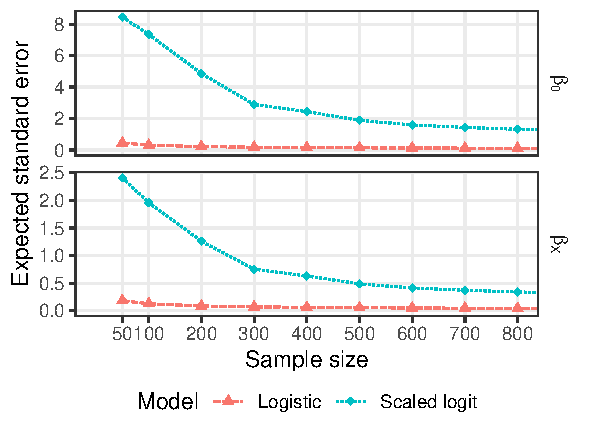
\includegraphics[width=0.69\textwidth]{../logistic-plot/vary_nsam_se.pdf}
	\caption{
	Simulation results of fitting the standard logistic and the scaled logit models to the same simulated datasets. 10,000 datasets were simulated. Shown is the mean standard deviation (estimate of the expected standard error) of the $\beta$ regression estimates from the standard logistic (the solid line) and the scaled logit (the dashed line). Points indicate parameter values at which the simulations were performed.
	}
	\label{SclrSE}
\end{figure}

\begin{figure}[H]
	\centering
	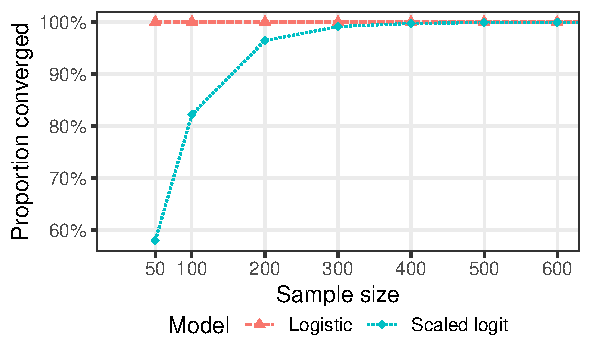
\includegraphics[width=0.69\textwidth]{../logistic-plot/vary_nsam.pdf}
	\caption{
	Simulation results of fitting the standard logistic and the scaled logit models to the same simulated datasets. 10,000 datasets were simulated. Shown is the proportion of successful attempts to fit the standard logistic (the solid line) and the scaled logit (the dashed line) model. Points indicate parameter values at which the simulations were performed.
	}
	\label{SclrConv}
\end{figure}
